\subsection{Gaussian Noise with Salt and Pepper}

By analyzing image 2 in an uniform area it can be seen that the image has both salt and pepper noise, illustrated in figure \ref{fig:hist2_uniform}.
As in section \ref{image_1} this is removed with a shifted median filter. 
It was found that a 5x5 filter removed the extreme values but was not efficient at removing the rest of the noise.

Thus a harmonic mean filter is used to remove the remaining salt noise.

Gaussian noise remains and this was removed with a homomorphic bilatteral filter.

The end result lacks contrast, which can be added with a histogram equalization scheme.
The histogram equalization stretches the color values to the extremes and thus the image quality does not improve.
So before the histogram equalization, a alpha trimmed mean with the kernel size of 7x7 and mean width of 3 is applied to remove further extreme values.

\begin{figure}[H]
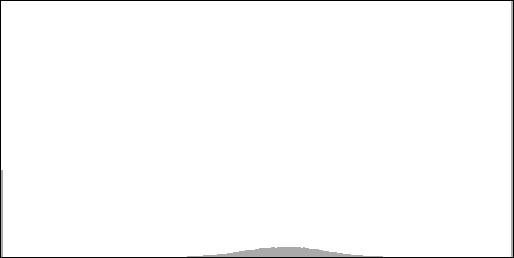
\includegraphics[width = 0.8 \linewidth]{graphics/hist2_uniform.png}
\caption{Histogram of the original ``Image2.png'' showing salt and pepper noise in a uniform area.}
\label{fig:hist_pepper}
\end{figure}
